\documentclass[a4paper, oneside]{report}
\usepackage{graphicx}
\DeclareGraphicsExtensions{.pdf,.png,.jpg}
\usepackage{blindtext}
\usepackage{tabularx}
\usepackage[english]{babel}
\begin{document}
	\setlength{\arrayrulewidth}{0.5mm}
	\setlength{\tabcolsep}{18pt}
	\renewcommand{\arraystretch}{1.5}
\chapter*{Building Gene Regulatory Network: experimental approach}
\section*{Introduction}

Developmental gene regulatory networks (dGRNs) plays a crucial role in the development of every single individual, especially multicellular. 
They regulate developmental processes not only during embryogenesis, but also affect post-embrionic morphogenetic processes like regeneration, asexual reproduction and growth.

GRN can be viewed as highly complicated network of protein-gene interactions. 
As a proteins in most of the cases act transcription factors (TFs). 
TFs are the proteins which has special DNA-binding motifs in their structure. 
This allows them to bind to regulatory elements in adjacent to gene regions (cis-regulatory modules) and regulate gene expression.
Depending on type of the interaction (activation/repression) there are can be several outcomes.
If TF binds to enchancer region, gene expression increase.
Opposite to that, if protein binds to silencer region then gene decrease its expression.
Also there can be more complicated types of interaction. 
For example protein could be insulator, enhancer-blocker or a barrier.
As a result most of the processes during development can be seen as complex network with lots of different gene-protein interactions.
Such networks usually illustrated using graphs.  
Nodes shows genes, TFs or signal molecules, edges illustrate types of interaction.
Such graphs in some cases reach vary big complexity.
As a consequense arise a questions: how can we reconstruct such networks? 
What kind of data should we use? 
And what are the potencial outcomes from reasearch of such gene interactions?

The purpose of this review was to demonstrate different approaches in building gene regulatory networks.
Special attention was paid to developmental GRNs.  

\section*{Developmental gene regulatory networks}

Term \textbf{\textit{developmental gene regulatory networks}} (dGRNs) was first introduced by E. H. Davidson.
Usually this term refers to a GRN which preferentially consists of genes crucial for the development. 

\begin{figure}[h]
\center{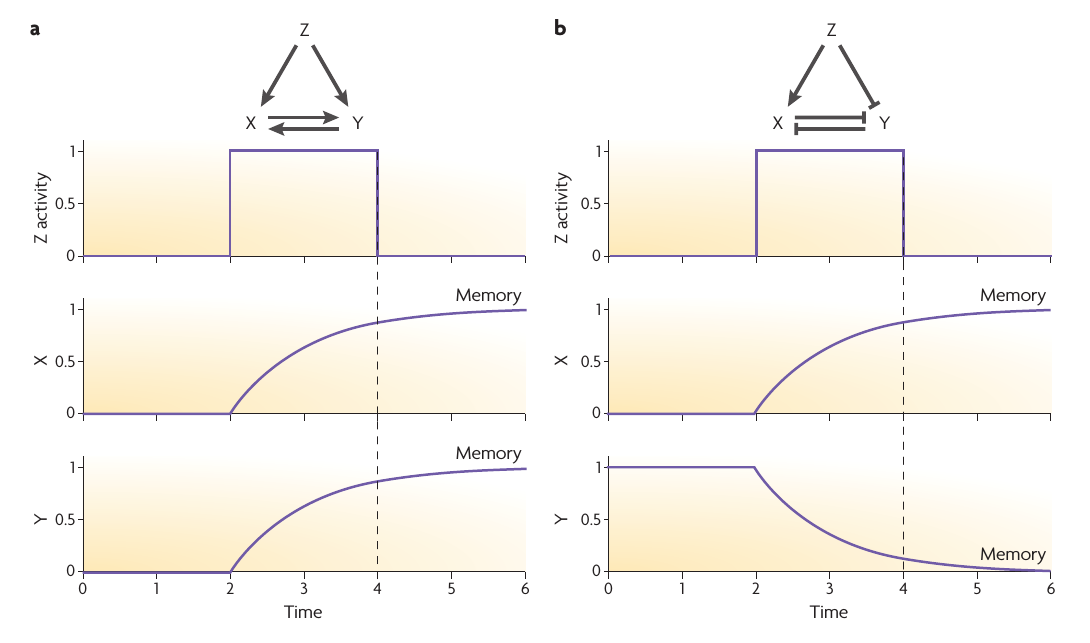
\includegraphics[width=1\linewidth]{fig_1}}
\caption{Two types of positive-feedback loops. Graph with curves represent activity (mRNA concentration) of the X,Y and Z genes. 
a | Network motifs with a double-positive-feedback loop.
b | Regulated feedback with a double-negative-feedback loop.}
\end{figure}

Developmental GRNs share lots of common features with other types of gene networks \cite{Alon2007}.
For example lots of networks typically has the same recurring regulation patterns as positive autoregulation (PAR), negative autoregulation (NAP), feedforward loops (FFLs) etc.
This common patterns called \textbf{\textit{network motifs}}.
It is recurring circuits of interactions from which the gene networks are built.
Also usually GRNs have hierarchical structure \cite{Erwin2009}.
It means that those genes that control the initial stages of development are at the top of the hierarchy and those genes that execute the detailed functions of cell differentiation are at the periphery.
Consequently, changes in upstream genes have far larger effect than in downstream.
For example changes in gap genes in early development of \textit{Drosofila melanogaster} have more impact on final body plan than changes in genes which regulate eyes pigmentation.
There are lots of others similarities.
But at the same time developmental GRNs have their own characteristic features.

First of all, they tend to have longer cascades than some other GRNs.
It can be explained by the role of this cascades.
Often they require transduce signal through the whole process of development, through lots of cell generations.
That is why timescale of such process is very slow.
Sometimes it is one cell generation at each cascade step.
And that brings us to the second characteristic feature of developmental GRNs.
They can functioning even after input signal has vanished.
The signal can be inherited during cell division and subsequently be transduced to next cell generations.
In this case often used repressor cascades, since they are more tolerant to concentration biases of signal molecule.
Such signal inheritance occures because of \textbf{\textit{positive-feedback loops}} (PFLs).
PFL is a process in which two events are mutually reinforcing each other.
There are two kind of PFLs: double-positive loop and a double-negative loop (fig. 1).

\begin{figure}[h]
	\center{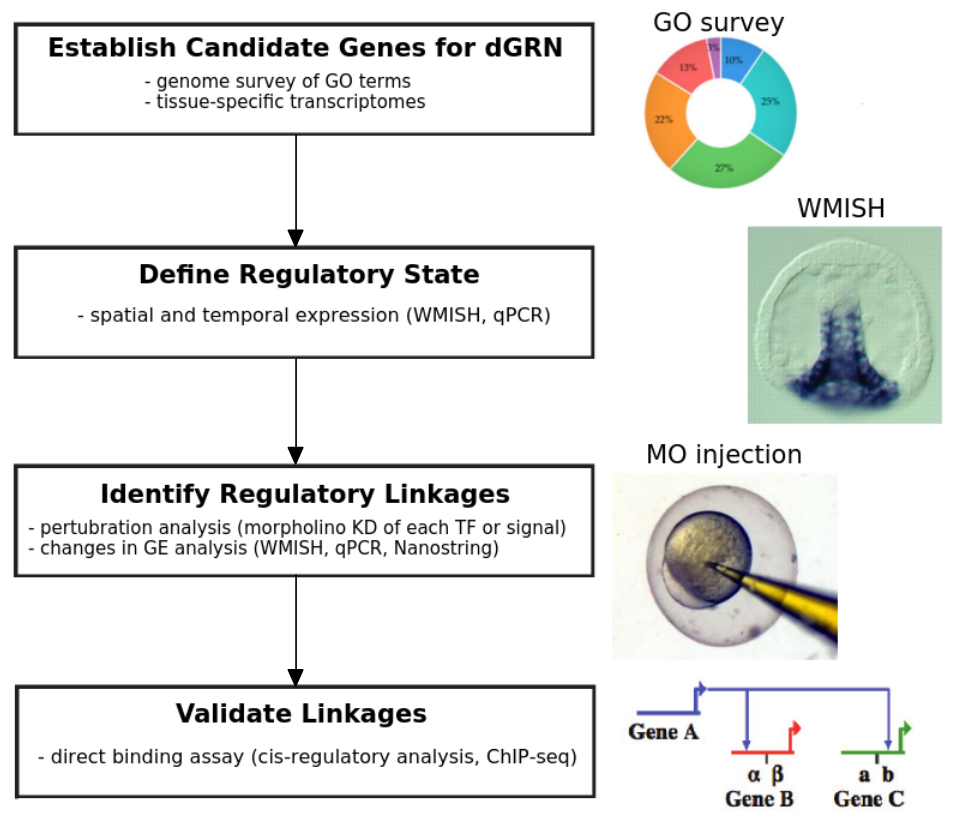
\includegraphics[width=1\linewidth]{fig_2}}
	\caption{Steps in construction and validation of developmental gene regulatory networks (dGRNs).}
\end{figure}

In doble-positive-feedback loop (fig.1a) when signal molecule Z is activated, proteins X and Y begin to be produced. 
After that X and Y develop self-sustained loop and mutually activate each other.
So than even if Z is discarded (dashed line), loop A-B continue existinig.

In doble-negative-feedback loop (fig.2a), initially, there is a high concentration of Y and it represes X.
After Z is activated, X is produced and Y is repressed.
As a result after deactivation of Z (dashed line) signal is transduced by X.
Y at the same moment is discarded.
Thus, the feedback implements a memory.
And that is how dGRNs transduce signal after vanishing of signal input.

Because of these features study of dGRNs has several difficulties.
As we now understand in study of developmnent we always deal with dynamic biological systems.
That is why researcher have to monitor multiple time points.
Moreover he has to understand the start and the end point of studied process.

Next we discuss how solve such difficulties and try to review common technologies which is involved in GRN building.   

\section*{Experiment}

In order to build GRN related to any development process we need to answer the following questions:

\vspace{2mm}

1) What TFs or signal molecules are participate in the process? 

2) When do genes of those factors express? (Temporal expression)

3) Where do that happens? (Spatial expression)

4) And how they interact with each other?

\vspace{2mm}

We can distinguish two main approaches in building GRN. First is exprimental approch. In this way we predominantly operate experimental data (microarrays, qPCR, hybridization \textit{in situ}, morphology etc). Second is computation approach where modeling of GRN is based on some descriptive and mathematical models using already generated data. In this review we will concentrate on first approach. In subsequent literature reviews we will cover second approach.

\subsection*{Regulatory genes identification}

The first step in building GRNs is regulatory genes identification.
If complete genome of the organism is available, than the best way is  genome-wide survey with identification of all predicted regultory genes.
Regulatory genes predominantly very conserved.
Therefore, transcription factors and signal molecules encoded by the regulatory genome can be identified by sequence-based homology searching using BLAST. 
Also DNA-binding motifs can help identify potencial TF.
The next step after identification of the majority of regulatory genes is to revel when and where this genes are expressed.


\begin{table}
	\makebox[\textwidth]{%
	\begin{tabular}{p{14cm}}
		\hline
		\textbf{Temporal restriction}
		\\
		\hline
		
		\textbf{a.} Direct transcriptional activation requires coincident expression of driver and target or driver expression earlier
		than targets
		
		\textbf{b.} Direct activation by ligand-binding in the recipient cells requires that the downstream genes not be expressed
		prior to the ligand
		\\
		\hline
		\textbf{Spatial restriction}
		\\
		\hline
		
		\textbf{a.} Direct transcriptional activation possible when driver and target are co-expressed in same domain
		
		\textbf{b.} Indirect interaction through signal(s) is implied if effect is observed in the domain in which the perturbed gene
		is not expressed
		
		\textbf{c.} Direct transcriptional repression requires that the repressor and its targets not overlap in their expression
		domain, or in the same domain at successive developmental stages
		\\
		\hline
		\textbf{Parsimonious topology}
		\\
		\hline
		
		\textbf{a.} Direct target of a transcription factor is more strongly affected than indirect targets
		
		\textbf{b.} A given interaction is presumed indirect if identified direct linkages suffice to explain the data
		\\
		\hline
		\textbf{Special linkages}
		\\
		\hline
		
		Double negative control logic is required when interference with a canonical repressor causes decrease in
		expression of target genes
		\\
		\hline
	
	\end{tabular}}
	
	\caption{Rules for Building Gene Regulatory Networks Based on Perturbation Data}	
\end{table}



\subsection*{Temporal expression}

At this stage, we encounter several problems.
Develppment is a longitudional event which takes lots of time.
Also it is highly dynamic serial event.
Thus, researcher have to chracterise this great multitude of RGs in different stages or conditions.
It is not a trivial task.
For this often use several methods:

\vspace{2mm}

1) Microarrays

2) qPCR 

3) NanoString 

\vspace{2mm}

When temporal expression of particular genes is identified, the next step is spatial expression revealing.

\subsection*{Spatial expression}

The most common and straight-forward way is hybridization \textit{in situ}.
This allows you reveal expression pattern of known regulatory gene.  
But unfortunatelly this stage is very time-consuming.
Additional combination with image analyzing techniaques allows one to achieve high resolution.
Mapping regulatory gene expression to various territorial domains is essential for subsequent analysis of the GRN.

\subsection*{Linkages}

\subsection*{Validation}

\subsection*{Visualisation}

\section*{Conslusion}


Therefore research of such a complex regulatory systems can shed more light on developmenatal processes and help in the curing of molecular genetic diseases associated with the violation of the networks.

\bibliographystyle{abbrv}
\bibliography{references}

\end{document}



